\section{Results}
\label{sec:results}

Looking at Figure \ref{fig:hovmullerSineBounded}, we see the time evolution of a sine wave in the bounded domain. The wave propagated towards the east, and we saw a clear distinction between phases.
\begin{figure}[htbp]
	\centering
	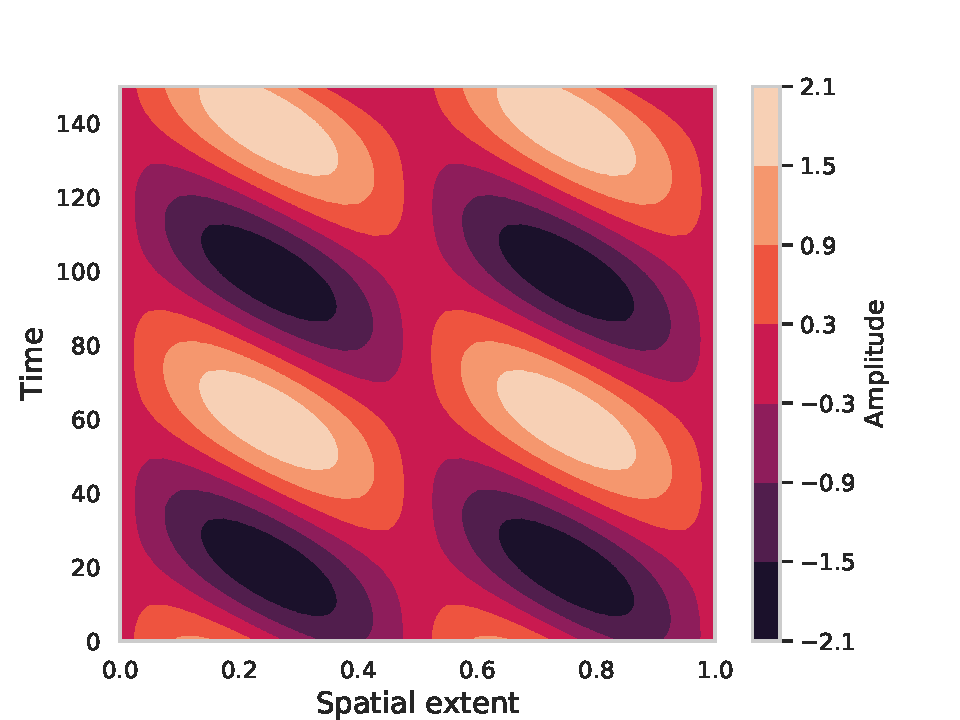
\includegraphics[width=0.5\textwidth]{hovmuller_boundedsine.pdf}
	\caption{Hov Müller diagram of a bounded Rossby wave with a initial sine wave using a explicit scheme.}
	\label{fig:hovmullerSineBounded}
\end{figure}

\begin{figure}[htbp]
	\centering
	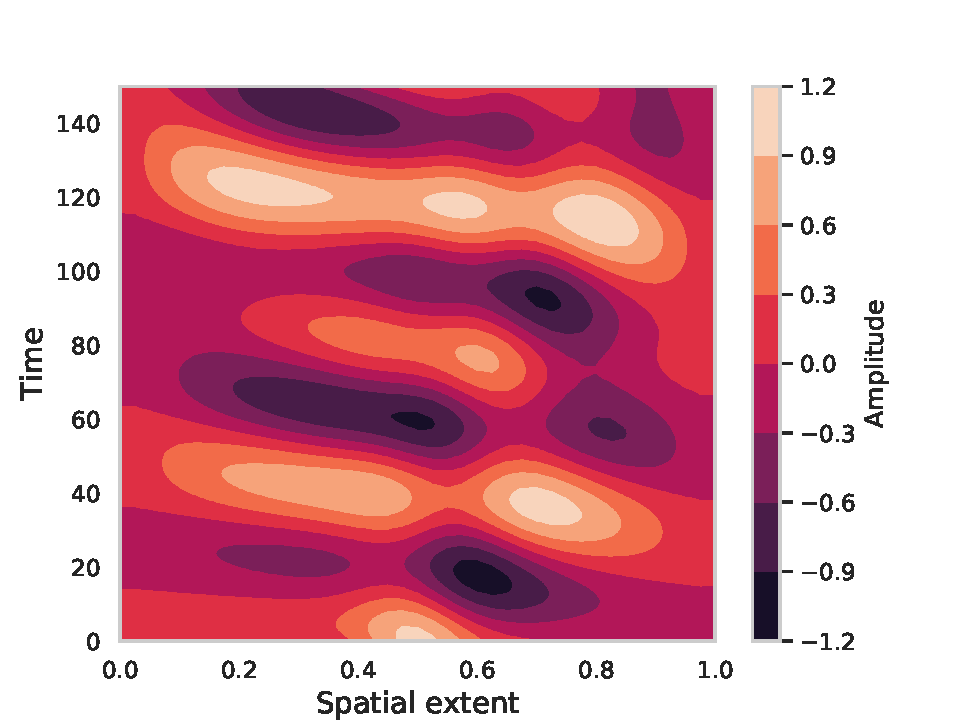
\includegraphics[width=0.5\textwidth]{hovmuller_boundedgaussian.pdf}
	\caption{Hov Müller diagram of a bounded Rossby wave initially a gaussian using a explicit scheme.}
	\label{fig:hovmullerGaussianBounded}
\end{figure}

\begin{figure}[htbp]
	\centering
	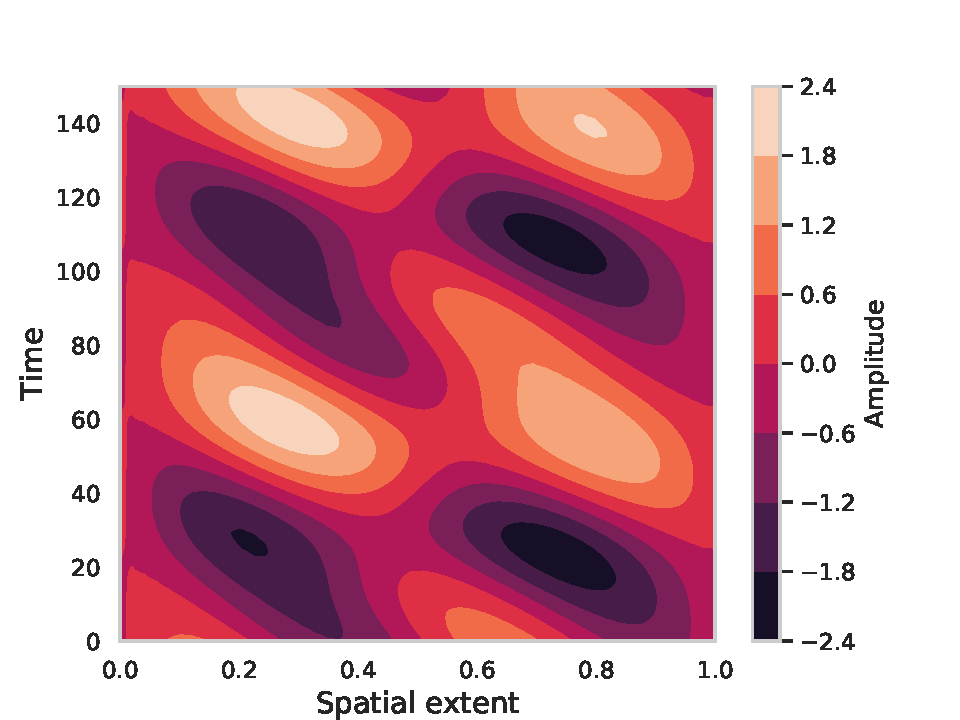
\includegraphics[width=0.5\textwidth]{hovmuller_periodicsine.pdf}
	\caption{Hov Müller diagram of a Rossby wave with periodic boundary conditions, initially a sine wave using a explicit scheme.}
	\label{fig:hovmullerSinePeriodic}
\end{figure}

\begin{figure}[htbp]
	\centering
	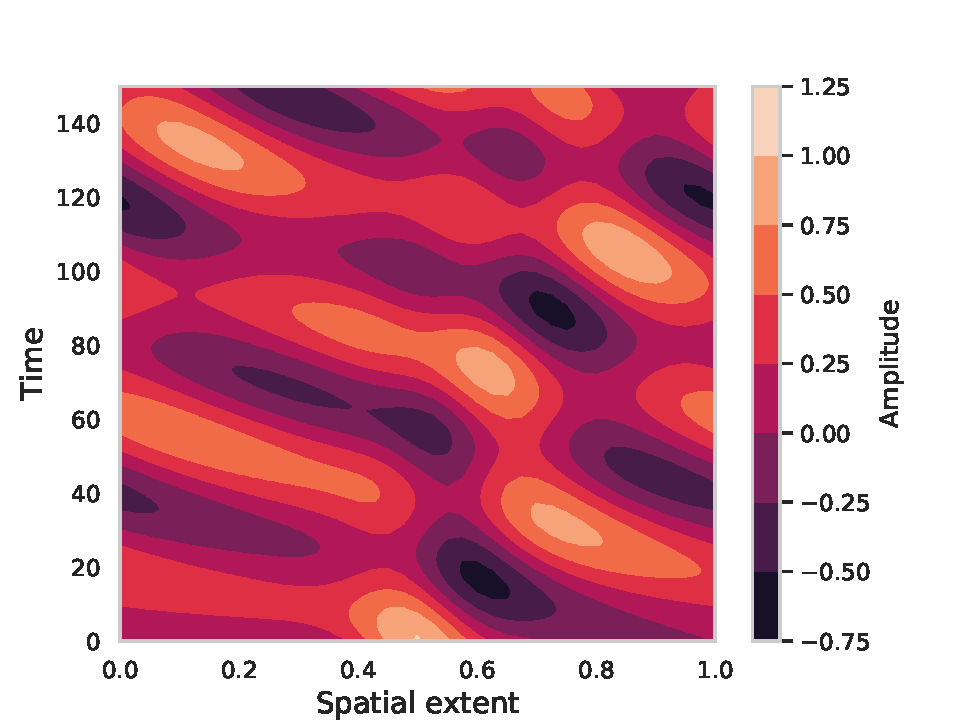
\includegraphics[width=0.5\textwidth]{hovmuller_periodicgaussian.pdf}
	\caption{Hov Müller diagram of a Rossby wave with periodic boundary conditions, initially a gaussian using a explicit scheme.}
	\label{fig:hovmullerGaussianPeriodic}
\end{figure}

\begin{table}[htbp]
	\centering
	\begin{tabular}{lrr}
		\textbf{n} & $\mathbf{{t_g}/{t_s}}$ & $\mathbf{{t_{LU}}/{t_s}}$  \\
		\midrule
		\addlinespace[0.1cm]

		10         & 2.08                                                                                          & 3.70                                                                                        \\
		$10^2$       & 1.89                                                                                          & $1.00\cdot 10^2 $                                                                                         \\
		$10^3$       & 1.48                                                                                          & $1.05 \cdot 10^4 $                                                                                        \\
		$10^4$       & 1.43                                                                                          & $1.18 \cdot 10^6$                                                                                         \\
		$10^5$       & 1.39                                                                                          & -                                                                                         \\
		$10^6$       & 1.41                                                                                          & -                                                                                        \\
		$10^7$       & 1.39                                                                                          &    -
	\end{tabular}  \caption{Ratio between CPU time for the general algorithm ($\mathbf{t_g}$), the special algorithm ($\mathbf{t_g}$) and the LU decomposition algorithm ($\mathbf{t_{LU}}$) for different matrix sizes (\textbf{n}). The LU decomposition crashed for \textbf{n} greater than $10^4$.} \label{table:time}
\end{table}
